\documentclass[xcolor=dvipsnames]{beamer}
\usepackage[T1]{fontenc}
\usepackage[utf8]{inputenc}
\usepackage[english,slovak]{babel}

\usepackage{amsmath}
\usepackage{amsthm}
\usetheme{Pittsburgh}
\useoutertheme{shadow}

\usepackage{graphicx}
\usepackage{caption}
\usepackage{subcaption}
\captionsetup{compatibility=false}

\usepackage{tabularx}

% \usepackage{movie15}
\usepackage{tikz}



\usepackage{listings}
\lstloadlanguages{Ruby}
\lstset{%
basicstyle=\ttfamily\color{black},
commentstyle = \ttfamily\color{red},
keywordstyle=\ttfamily\color{blue},
stringstyle=\color{orange}}

\usetheme{Warsaw}

\setbeamercolor{normal text}{fg=white,bg=black!90}
\setbeamercolor{structure}{fg=white}

\setbeamercolor{alerted text}{fg=red!85!black}

\setbeamercolor{item projected}{use=item,fg=black,bg=item.fg!35}

\setbeamercolor*{palette primary}{use=structure,fg=structure.fg}
\setbeamercolor*{palette secondary}{use=structure,fg=structure.fg!95!black}
\setbeamercolor*{palette tertiary}{use=structure,fg=structure.fg!90!black}
\setbeamercolor*{palette quaternary}{use=structure,fg=structure.fg!95!black,bg=black!80}

\setbeamercolor*{framesubtitle}{fg=white}

\setbeamercolor*{block title}{parent=structure,bg=black!60}
\setbeamercolor*{block body}{fg=black,bg=black!10}
\setbeamercolor*{block title alerted}{parent=alerted text,bg=black!15}
\setbeamercolor*{block title example}{parent=example text,bg=black!15}



%-------------------------------------------------------------------------------------
\title{\bf Aeris - Hybrid multirobotics system}
\author{Michal CHOVANEC et. al }

%\\Faculty of management science and informatics}

\date[EURP]{\it April 2016}



\begin{document}

\usebackgroundtemplate{
\tikz[overlay,remember picture] \node[opacity=0.99, at=(current page.center)] {
   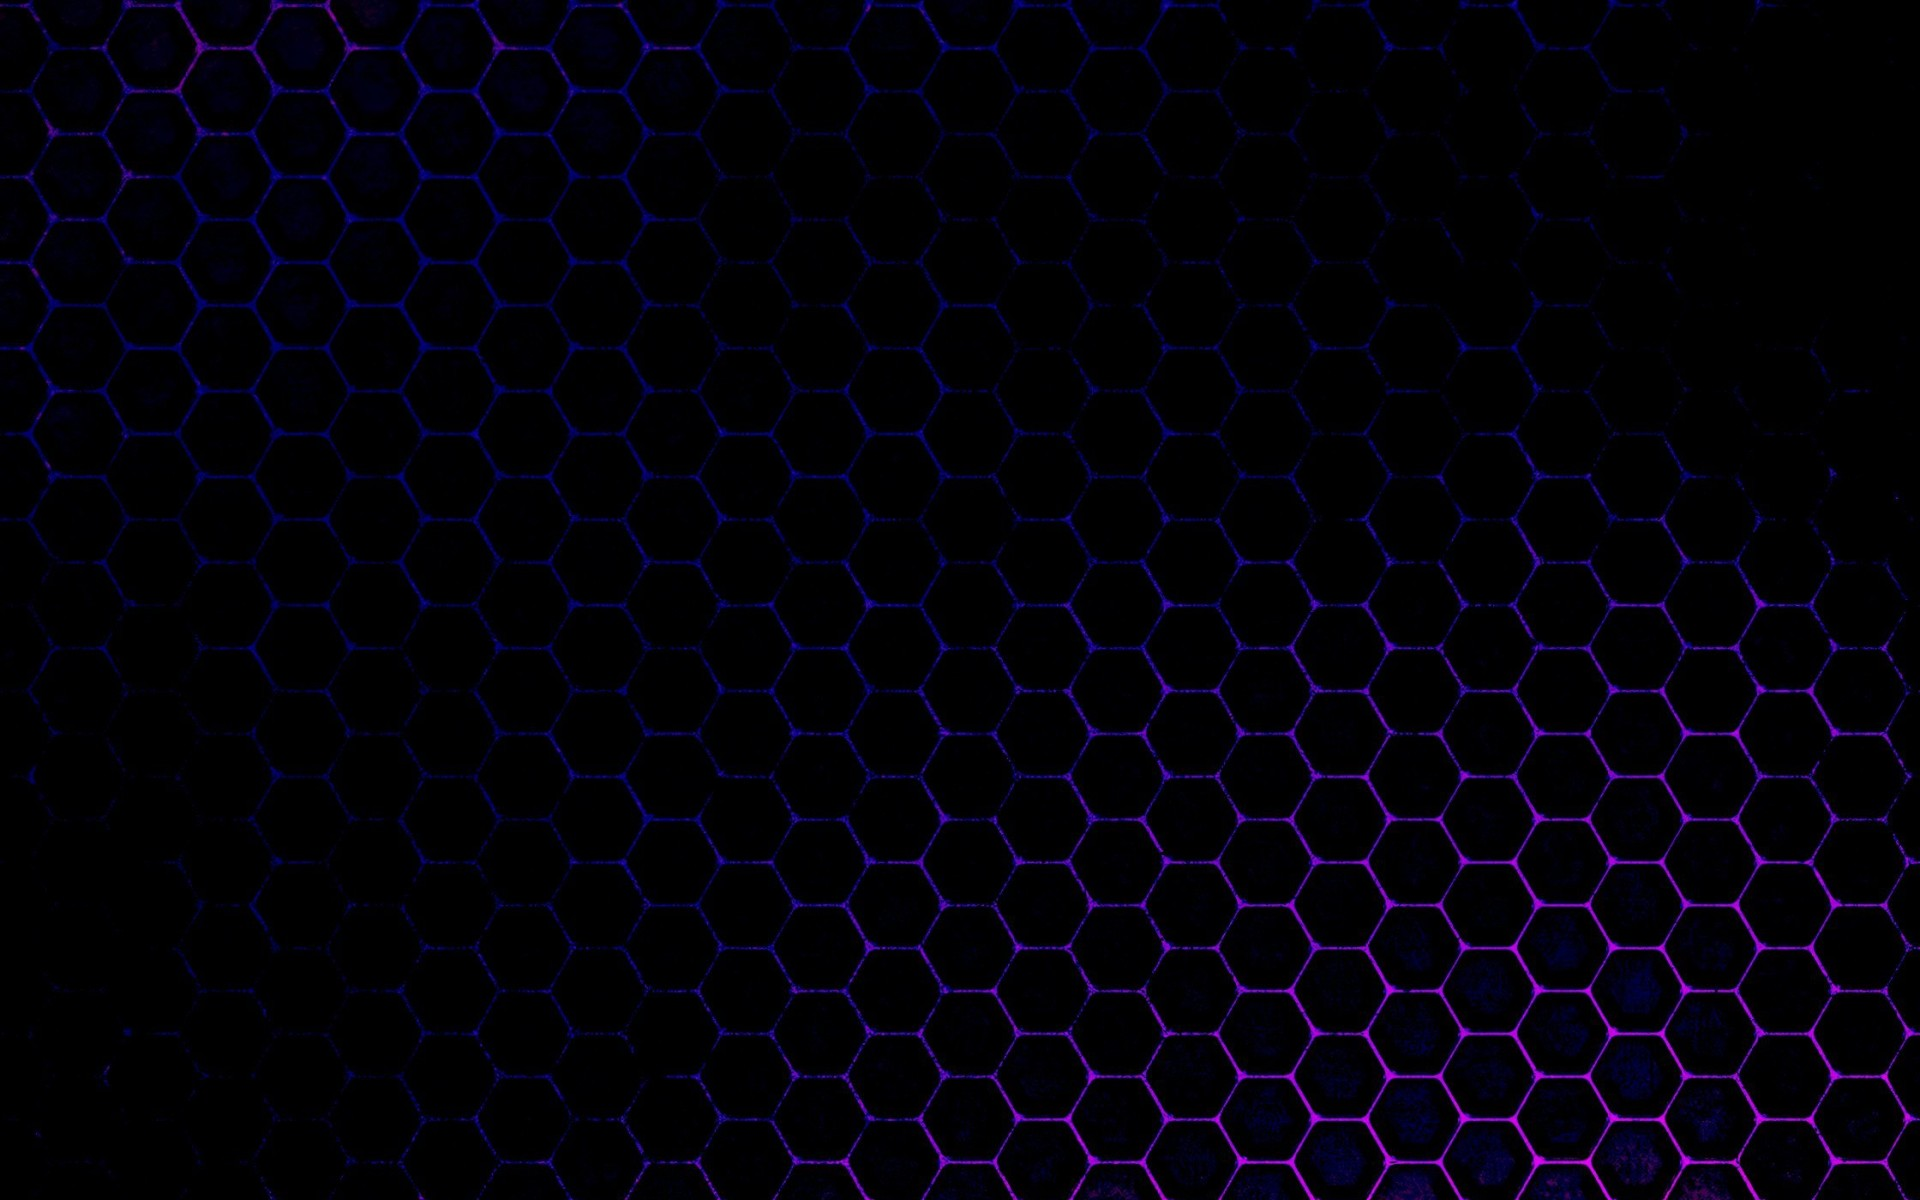
\includegraphics[height=\paperheight,width=\paperwidth]{back.jpg}};
}
\begin{frame}
\titlepage
\end{frame}

%\usebackgroundtemplate{ }
\begin{frame}{\bf Combine virtual reality with real robots}

\begin{figure}[!htb]
\centering
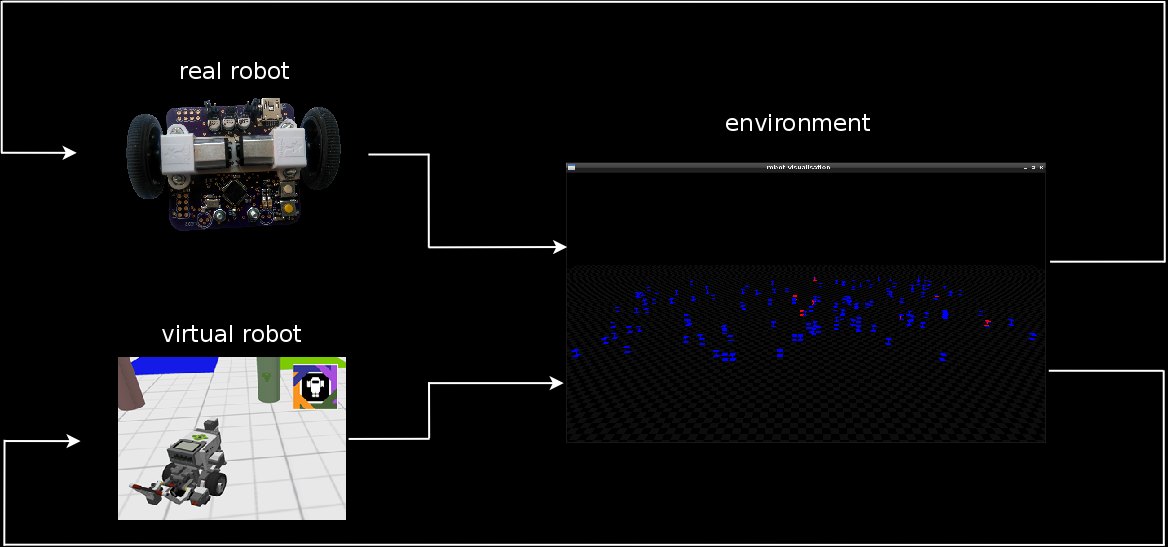
\includegraphics[scale=.2]{../diagrams/aeris_idea_inv.png}
\end{figure}

\begin{itemize}
  \item Real robot, based on ARM Cortex M4F
  \item Virtual robot, running on Linux PC
  \item Virtual environmnent, running on Linux PC
\end{itemize}


\end{frame}



%\usebackgroundtemplate{ }
\begin{frame}{\bf Comparsion with common solution}

\begin{minipage}{.5\textwidth}

\begin{figure}[!htb]
\centering

\includegraphics[scale=.23]{../diagrams/common_lab_inv.png}
\end{figure}

\begin{itemize}
  \item Seperated model and reality
  \item Different inputs for virtual and real robot
  \item Difficult to compare
\end{itemize}

  \end{minipage}%
\begin{minipage}{.5\textwidth}

\begin{figure}[!htb]
\centering

\includegraphics[scale=.23]{../diagrams/hybrid_lab_inv.png}
\end{figure}

  \begin{itemize}
    \item Single environment
    \item Same inputs for virtual and real robot
    \item Easy comparable
  \end{itemize}

\end{minipage}

\end{frame}




\begin{frame}{\bf Aeris system photo}

Linefollower on dynamic changing line

\begin{figure}[!htb]
\centering
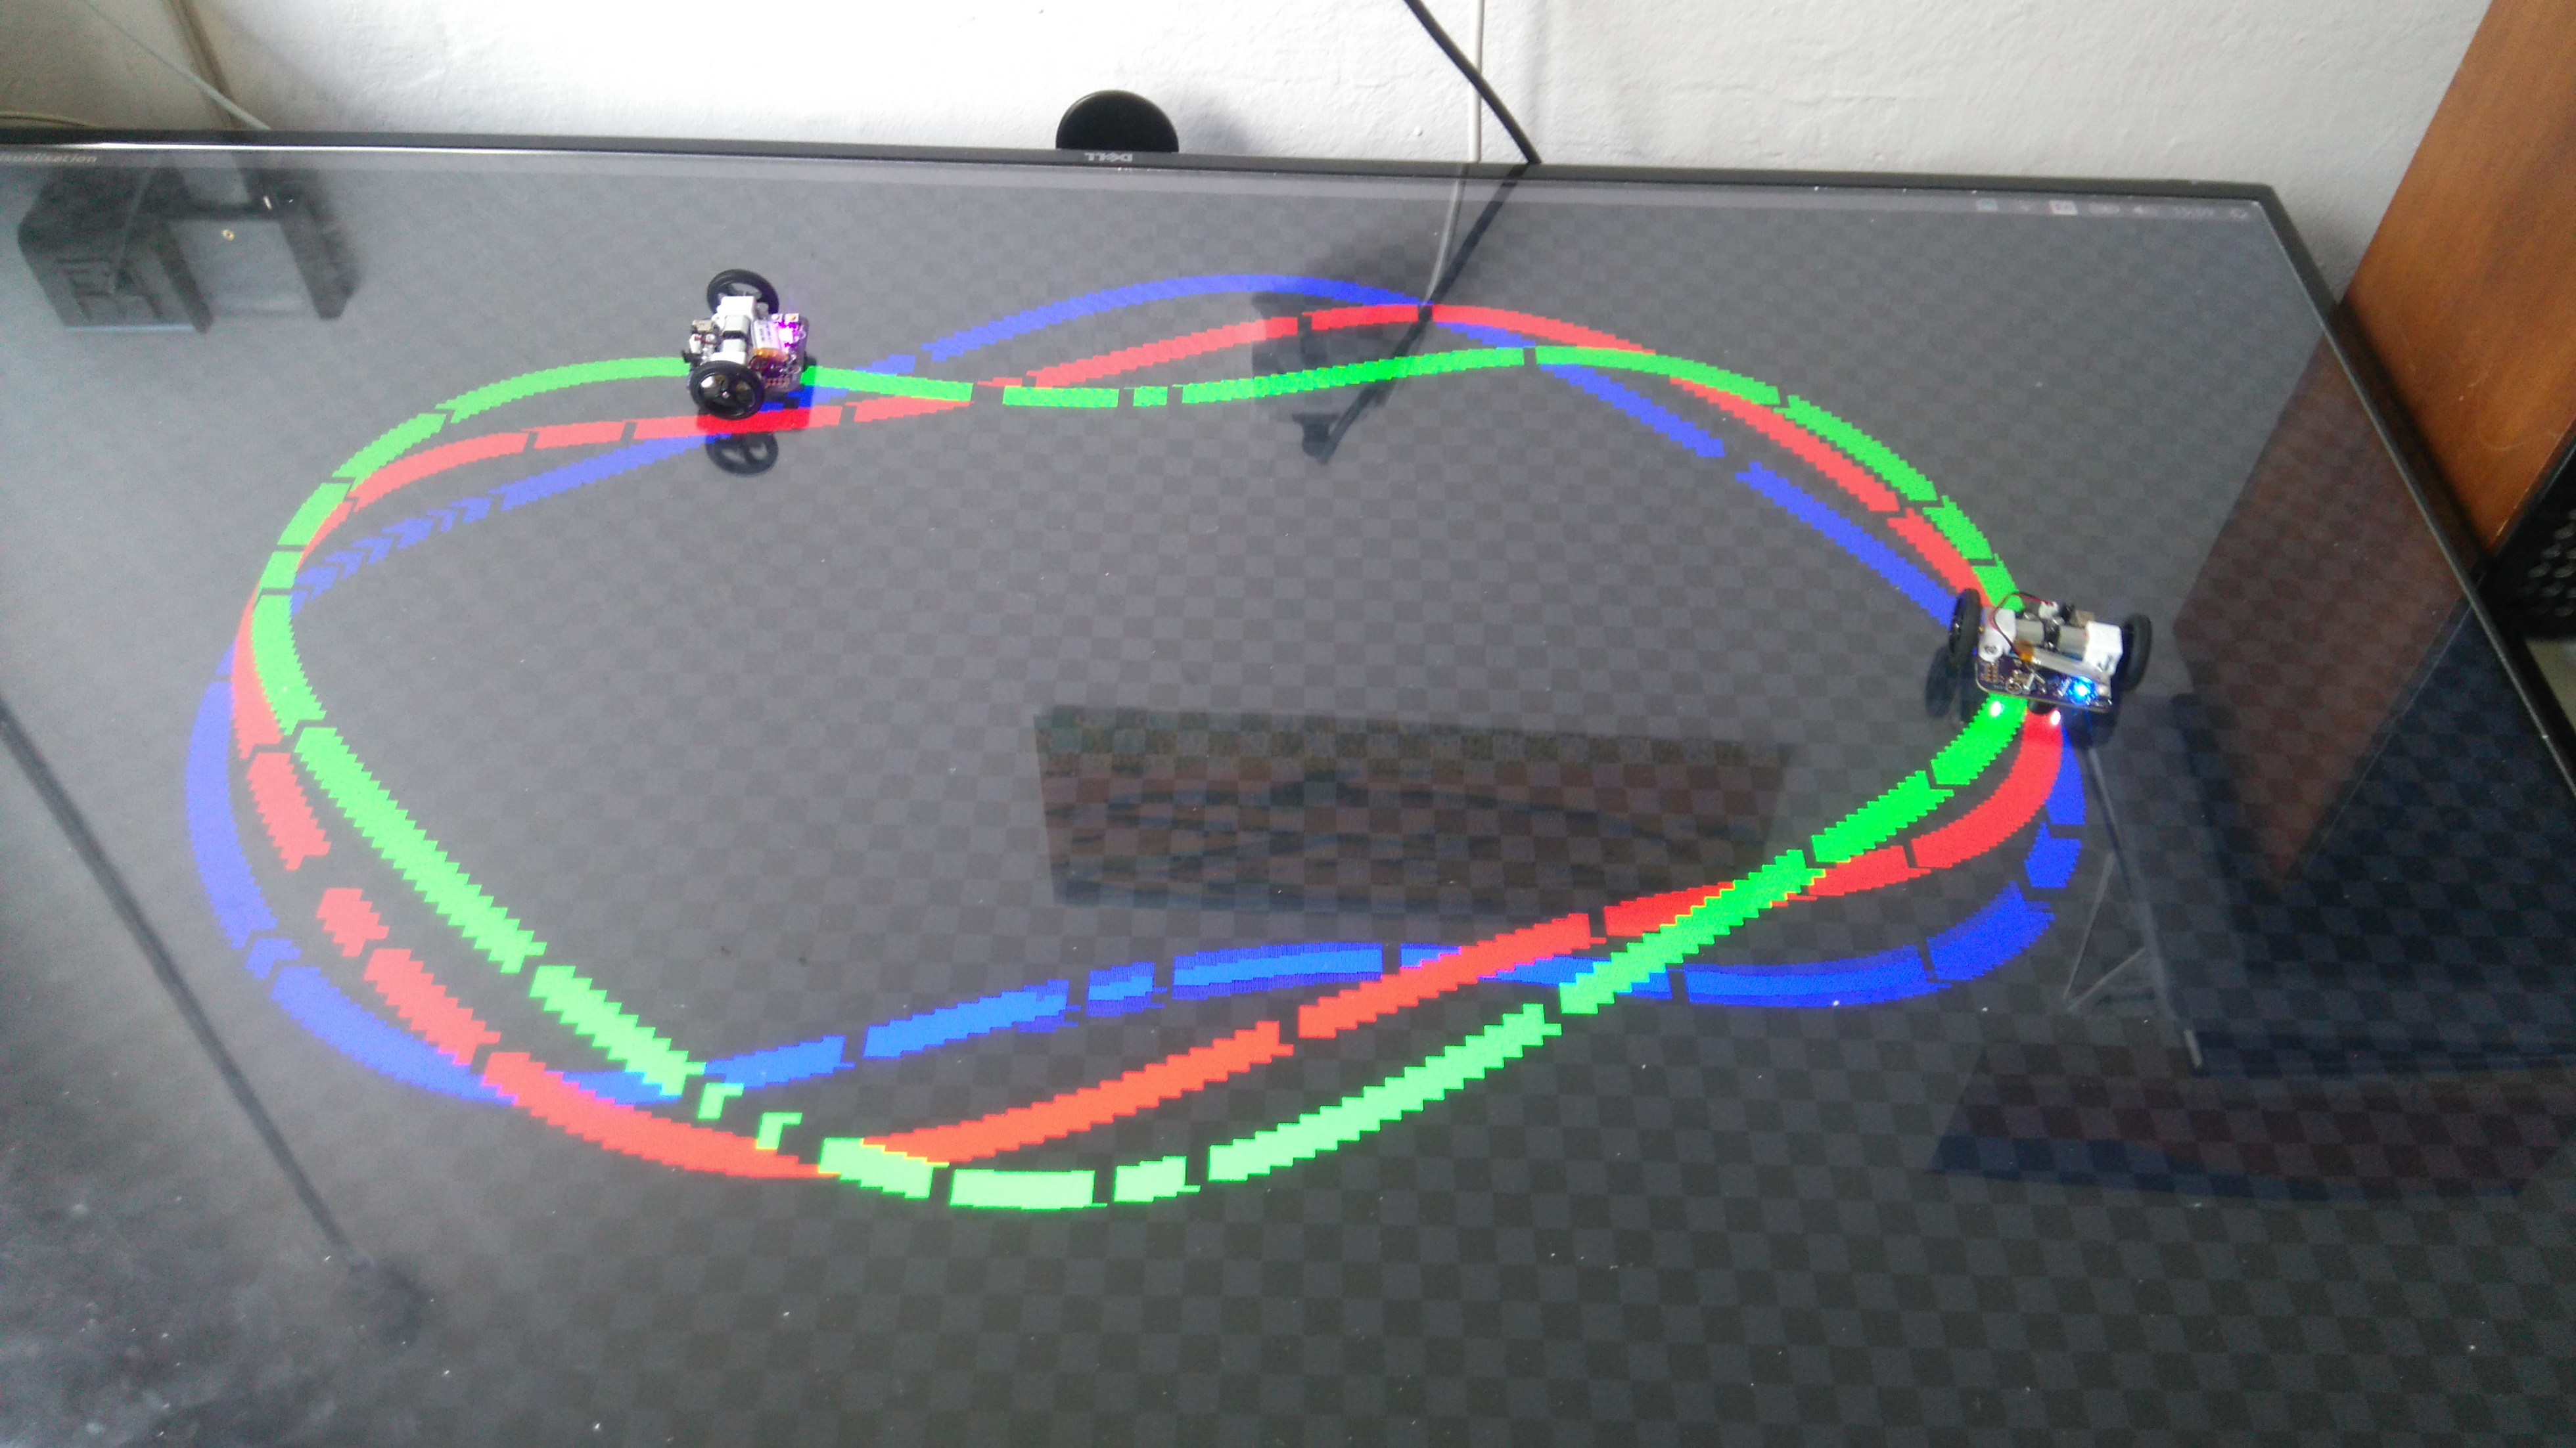
\includegraphics[scale=.07]{../pictures/line_follower.jpg}
\end{figure}

\end{frame}




\begin{frame}{\bf Software architecture}

\begin{figure}[!htb]
\centering

\includegraphics[scale=.3]{../diagrams/aeris_software_block_inv.png}
\end{figure}


\begin{minipage}{.5\textwidth}


\begin{itemize}
  \item C++ 11, GNU Linux
  \item client-server
  \item OpenGL
\end{itemize}

  \end{minipage}%
\begin{minipage}{.5\textwidth}

  \begin{itemize}
    \item Server, Visualisation, Robots
    \item each on own computer
    \item multiple visualisations
    \item html5 visualisation
  \end{itemize}

\end{minipage}


\end{frame}


\begin{frame}{\bf Robot hardware}

\begin{minipage}{.5\textwidth}

\begin{itemize}
  \item 72MHz ARM Cortex M4 with FPU
  \item IMU : gyroscope, compass, accelerometer
  \item 4x RGB surface sensors
  \item USB programming  and charging
  \item WiFi and I2C expansion connectors
  \item 2x DC motors
\end{itemize}

  \end{minipage}%
\begin{minipage}{.5\textwidth}

  \begin{figure}[!htb]
  \centering
  \includegraphics[scale=.04]{../pictures/desc_top_mask.png}
  \end{figure}

\end{minipage}

\end{frame}



\begin{frame}{\bf Robot hardware}

\begin{minipage}{.5\textwidth}

\begin{itemize}
  \item 72MHz ARM Cortex M4 with FPU
  \item IMU : gyroscope, compass, accelerometer
  \item 4x RGB surface sensors
  \item USB programming  and charging
  \item WiFi and I2C expansion connectors
  \item 2x DC motors
\end{itemize}

  \end{minipage}%
\begin{minipage}{.5\textwidth}

  \begin{figure}[!htb]
  \centering
  \includegraphics[scale=.04]{../pictures/desc_bottom_mask.png}
  \end{figure}

\end{minipage}

\end{frame}


\begin{frame}{\bf Experiments}

\begin{minipage}{.5\textwidth}

\begin{itemize}
  \item Ant colony - pheromone footprint
  \item Virtual maze solving
  \item Line follower
  \item Self organizing systems
  \item Any problem asking for changing environment in time
    \begin{itemize}
      \item minisumo
      \item robotic football
      \item capture-the-flag game
      \item ...
    \end{itemize}

\end{itemize}

  \end{minipage}%
\begin{minipage}{.5\textwidth}

  \begin{figure}[!htb]
  \centering
  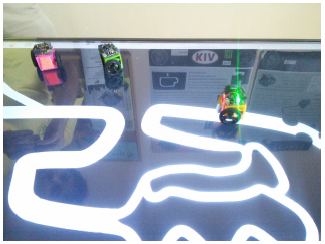
\includegraphics[scale=.5]{../pictures/aeris_photo_01.png}
  \end{figure}

\end{minipage}

\end{frame}




\begin{frame}{\bf Thanks you  for your attention}

\begin{itemize}
  \item web http://www.fribot.sk
  \item sources https://github.com/michalnand/aeris
\end{itemize}

Authors : Michal Chovanec, Lukas Cechovic, Lukas Mandak

\end{frame}










\end{document}
